\documentclass{standalone}
\usepackage{tikz}
\usetikzlibrary{patterns, positioning}


\begin{document}
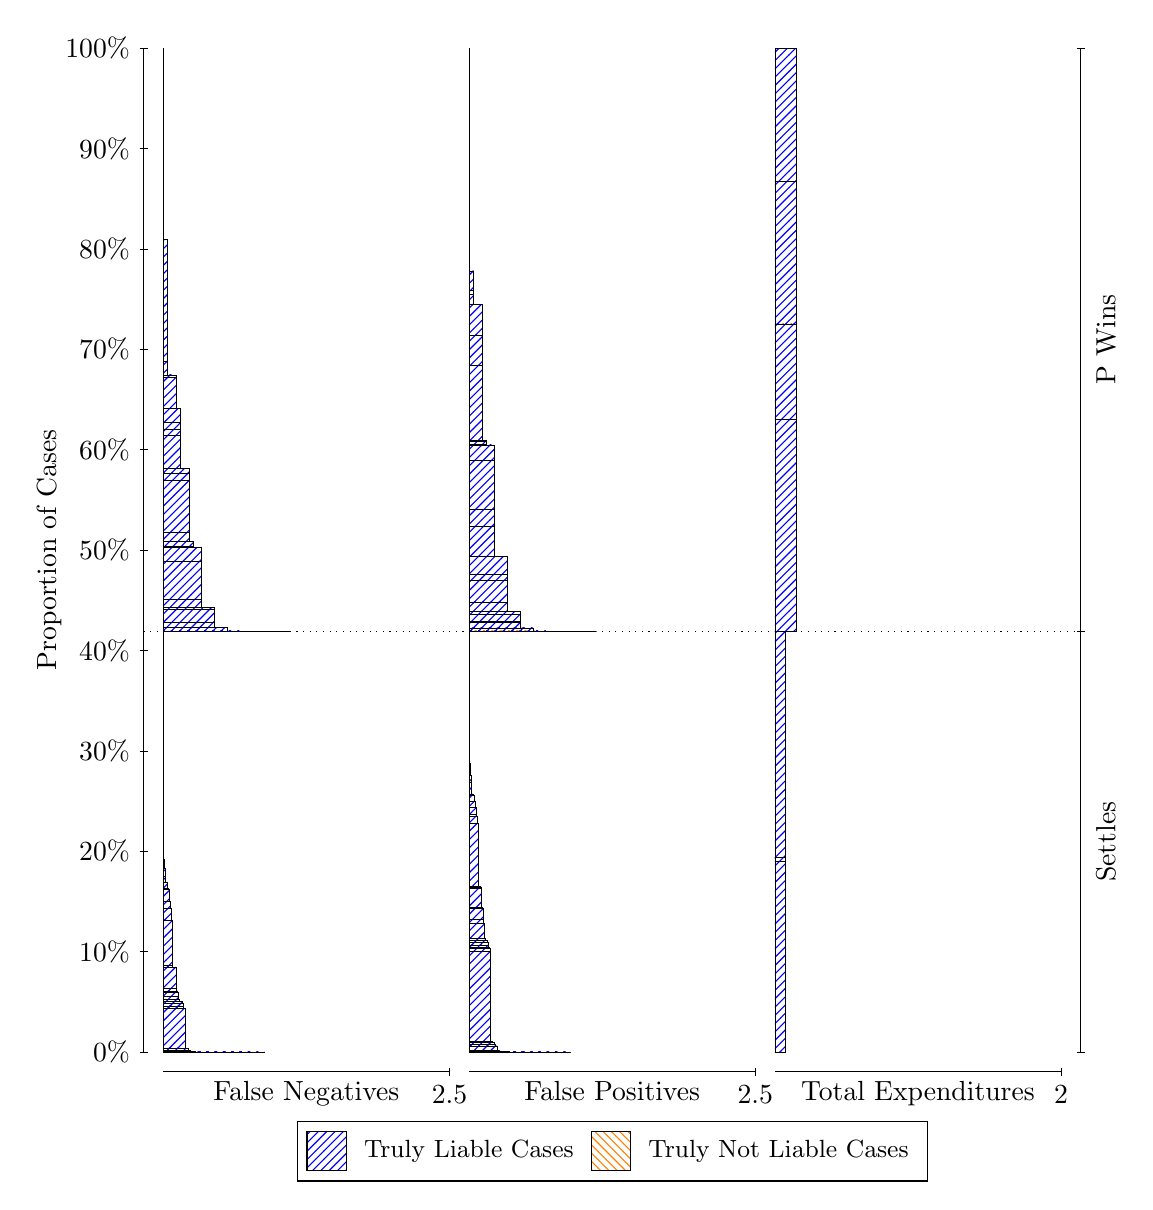
\begin{tikzpicture}
\draw[black, very thin] (1.5,1.75) -- (1.5,14.5);
\node[rotate=90, text=black, anchor=center] at (0.3, 8.125) {Proportion of Cases};
\draw[black, very thin] (1.45,1.75) -- (1.55,1.75);
\node[text=black, anchor=east] at (1.45, 1.75) {0\%};
\draw[black, very thin] (1.45,3.025) -- (1.55,3.025);
\node[text=black, anchor=east] at (1.45, 3.025) {10\%};
\draw[black, very thin] (1.45,4.3) -- (1.55,4.3);
\node[text=black, anchor=east] at (1.45, 4.3) {20\%};
\draw[black, very thin] (1.45,5.575) -- (1.55,5.575);
\node[text=black, anchor=east] at (1.45, 5.575) {30\%};
\draw[black, very thin] (1.45,6.85) -- (1.55,6.85);
\node[text=black, anchor=east] at (1.45, 6.85) {40\%};
\draw[black, very thin] (1.45,8.125) -- (1.55,8.125);
\node[text=black, anchor=east] at (1.45, 8.125) {50\%};
\draw[black, very thin] (1.45,9.4) -- (1.55,9.4);
\node[text=black, anchor=east] at (1.45, 9.4) {60\%};
\draw[black, very thin] (1.45,10.675) -- (1.55,10.675);
\node[text=black, anchor=east] at (1.45, 10.675) {70\%};
\draw[black, very thin] (1.45,11.95) -- (1.55,11.95);
\node[text=black, anchor=east] at (1.45, 11.95) {80\%};
\draw[black, very thin] (1.45,13.225) -- (1.55,13.225);
\node[text=black, anchor=east] at (1.45, 13.225) {90\%};
\draw[black, very thin] (1.45,14.5) -- (1.55,14.5);
\node[text=black, anchor=east] at (1.45, 14.5) {100\%};

\draw[black, very thin] (13.4,1.75) -- (13.4,14.5);
\draw[black, very thin] (13.35,1.75) -- (13.45,1.75);
\node[anchor=west] at (13.35, 1.75) {};
\draw[black, very thin] (13.35,7.0927) -- (13.45,7.0927);
\node[anchor=west] at (13.35, 7.0927) {};
\draw[black, very thin] (13.35,14.5) -- (13.45,14.5);
\node[anchor=west] at (13.35, 14.5) {};

\draw[black, very thin, pattern color=blue, pattern=north east lines] (1.75,1.75) rectangle (3.0398,1.75);
\draw[black, very thin, pattern color=blue, pattern=north east lines] (1.75,1.75) rectangle (2.9672,1.75);
\draw[black, very thin, pattern color=blue, pattern=north east lines] (1.75,1.75) rectangle (2.8945,1.75);
\draw[black, very thin, pattern color=blue, pattern=north east lines] (1.75,1.75) rectangle (2.8784,1.75);
\draw[black, very thin, pattern color=blue, pattern=north east lines] (1.75,1.75) rectangle (2.8218,1.75);
\draw[black, very thin, pattern color=blue, pattern=north east lines] (1.75,1.75) rectangle (2.8057,1.75);
\draw[black, very thin, pattern color=blue, pattern=north east lines] (1.75,1.75) rectangle (2.7492,1.75);
\draw[black, very thin, pattern color=blue, pattern=north east lines] (1.75,1.75) rectangle (2.733,1.75);
\draw[black, very thin, pattern color=blue, pattern=north east lines] (1.75,1.75) rectangle (2.7169,1.75);
\draw[black, very thin, pattern color=blue, pattern=north east lines] (1.75,1.75) rectangle (2.6765,1.75);
\draw[black, very thin, pattern color=blue, pattern=north east lines] (1.75,1.75) rectangle (2.6604,1.75);
\draw[black, very thin, pattern color=blue, pattern=north east lines] (1.75,1.75) rectangle (2.6442,1.75);
\draw[black, very thin, pattern color=blue, pattern=north east lines] (1.75,1.75) rectangle (2.6038,1.75);
\draw[black, very thin, pattern color=blue, pattern=north east lines] (1.75,1.75) rectangle (2.5877,1.75);
\draw[black, very thin, pattern color=blue, pattern=north east lines] (1.75,1.75) rectangle (2.5715,1.75);
\draw[black, very thin, pattern color=blue, pattern=north east lines] (1.75,1.75) rectangle (2.5554,1.75);
\draw[black, very thin, pattern color=blue, pattern=north east lines] (1.75,1.75) rectangle (2.5312,1.75);
\draw[black, very thin, pattern color=blue, pattern=north east lines] (1.75,1.75) rectangle (2.515,1.75);
\draw[black, very thin, pattern color=blue, pattern=north east lines] (1.75,1.75) rectangle (2.4989,1.75);
\draw[black, very thin, pattern color=blue, pattern=north east lines] (1.75,1.75) rectangle (2.4827,1.75);
\draw[black, very thin, pattern color=blue, pattern=north east lines] (1.75,1.75) rectangle (2.4585,1.75);
\draw[black, very thin, pattern color=blue, pattern=north east lines] (1.75,1.75) rectangle (2.4424,1.75);
\draw[black, very thin, pattern color=blue, pattern=north east lines] (1.75,1.75) rectangle (2.4262,1.75);
\draw[black, very thin, pattern color=blue, pattern=north east lines] (1.75,1.75) rectangle (2.4101,1.75);
\draw[black, very thin, pattern color=blue, pattern=north east lines] (1.75,1.75) rectangle (2.3939,1.75);
\draw[black, very thin, pattern color=blue, pattern=north east lines] (1.75,1.75) rectangle (2.3858,1.75);
\draw[black, very thin, pattern color=blue, pattern=north east lines] (1.75,1.75) rectangle (2.3697,1.75);
\draw[black, very thin, pattern color=blue, pattern=north east lines] (1.75,1.75) rectangle (2.3535,1.75);
\draw[black, very thin, pattern color=blue, pattern=north east lines] (1.75,1.75) rectangle (2.3374,1.75);
\draw[black, very thin, pattern color=blue, pattern=north east lines] (1.75,1.75) rectangle (2.3212,1.75);
\draw[black, very thin, pattern color=blue, pattern=north east lines] (1.75,1.75) rectangle (2.3132,1.75);
\draw[black, very thin, pattern color=blue, pattern=north east lines] (1.75,1.75) rectangle (2.297,1.75);
\draw[black, very thin, pattern color=blue, pattern=north east lines] (1.75,1.75) rectangle (2.2809,1.75);
\draw[black, very thin, pattern color=blue, pattern=north east lines] (1.75,1.75) rectangle (2.2647,1.7501);
\draw[black, very thin, pattern color=blue, pattern=north east lines] (1.75,1.7501) rectangle (2.2486,1.7501);
\draw[black, very thin, pattern color=blue, pattern=north east lines] (1.75,1.7501) rectangle (2.2405,1.7502);
\draw[black, very thin, pattern color=blue, pattern=north east lines] (1.75,1.7502) rectangle (2.2324,1.7507);
\draw[black, very thin, pattern color=blue, pattern=north east lines] (1.75,1.7507) rectangle (2.2244,1.7507);
\draw[black, very thin, pattern color=blue, pattern=north east lines] (1.75,1.7507) rectangle (2.2082,1.7507);
\draw[black, very thin, pattern color=blue, pattern=north east lines] (1.75,1.7507) rectangle (2.1921,1.7508);
\draw[black, very thin, pattern color=blue, pattern=north east lines] (1.75,1.7508) rectangle (2.1759,1.7509);
\draw[black, very thin, pattern color=blue, pattern=north east lines] (1.75,1.7509) rectangle (2.1678,1.7522);
\draw[black, very thin, pattern color=blue, pattern=north east lines] (1.75,1.7522) rectangle (2.1598,1.7542);
\draw[black, very thin, pattern color=blue, pattern=north east lines] (1.75,1.7542) rectangle (2.1517,1.7547);
\draw[black, very thin, pattern color=blue, pattern=north east lines] (1.75,1.7547) rectangle (2.1355,1.7548);
\draw[black, very thin, pattern color=blue, pattern=north east lines] (1.75,1.7548) rectangle (2.1194,1.7566);
\draw[black, very thin, pattern color=blue, pattern=north east lines] (1.75,1.7566) rectangle (2.1032,1.7585);
\draw[black, very thin, pattern color=blue, pattern=north east lines] (1.75,1.7585) rectangle (2.0952,1.7684);
\draw[black, very thin, pattern color=blue, pattern=north east lines] (1.75,1.7684) rectangle (2.0871,1.7715);
\draw[black, very thin, pattern color=blue, pattern=north east lines] (1.75,1.7715) rectangle (2.079,1.7737);
\draw[black, very thin, pattern color=blue, pattern=north east lines] (1.75,1.7737) rectangle (2.0709,1.7998);
\draw[black, very thin, pattern color=blue, pattern=north east lines] (1.75,1.7998) rectangle (2.0629,1.7999);
\draw[black, very thin, pattern color=blue, pattern=north east lines] (1.75,1.7999) rectangle (2.0467,1.8001);
\draw[black, very thin, pattern color=blue, pattern=north east lines] (1.75,1.8001) rectangle (2.0306,1.8031);
\draw[black, very thin, pattern color=blue, pattern=north east lines] (1.75,1.8031) rectangle (2.0225,2.3067);
\draw[black, very thin, pattern color=blue, pattern=north east lines] (1.75,2.3067) rectangle (2.0144,2.3086);
\draw[black, very thin, pattern color=blue, pattern=north east lines] (1.75,2.3086) rectangle (2.0064,2.3357);
\draw[black, very thin, pattern color=blue, pattern=north east lines] (1.75,2.3357) rectangle (1.9983,2.3682);
\draw[black, very thin, pattern color=blue, pattern=north east lines] (1.75,2.3682) rectangle (1.9902,2.3891);
\draw[black, very thin, pattern color=blue, pattern=north east lines] (1.75,2.3891) rectangle (1.9741,2.3921);
\draw[black, very thin, pattern color=blue, pattern=north east lines] (1.75,2.3921) rectangle (1.9579,2.4217);
\draw[black, very thin, pattern color=blue, pattern=north east lines] (1.75,2.4217) rectangle (1.9418,2.4513);
\draw[black, very thin, pattern color=blue, pattern=north east lines] (1.75,2.4513) rectangle (1.9337,2.5067);
\draw[black, very thin, pattern color=blue, pattern=north east lines] (1.75,2.5067) rectangle (1.9256,2.5272);
\draw[black, very thin, pattern color=blue, pattern=north east lines] (1.75,2.5272) rectangle (1.9175,2.5601);
\draw[black, very thin, pattern color=blue, pattern=north east lines] (1.75,2.5601) rectangle (1.9095,2.8276);
\draw[black, very thin, pattern color=blue, pattern=north east lines] (1.75,2.8276) rectangle (1.9014,2.8295);
\draw[black, very thin, pattern color=blue, pattern=north east lines] (1.75,2.8295) rectangle (1.8852,2.8313);
\draw[black, very thin, pattern color=blue, pattern=north east lines] (1.75,2.8313) rectangle (1.8691,2.8505);
\draw[black, very thin, pattern color=blue, pattern=north east lines] (1.75,2.8505) rectangle (1.861,3.4218);
\draw[black, very thin, pattern color=blue, pattern=north east lines] (1.75,3.4218) rectangle (1.8529,3.4269);
\draw[black, very thin, pattern color=blue, pattern=north east lines] (1.75,3.4269) rectangle (1.8449,3.5724);
\draw[black, very thin, pattern color=blue, pattern=north east lines] (1.75,3.5724) rectangle (1.8368,3.6667);
\draw[black, very thin, pattern color=blue, pattern=north east lines] (1.75,3.6667) rectangle (1.8287,3.8149);
\draw[black, very thin, pattern color=blue, pattern=north east lines] (1.75,3.8149) rectangle (1.8126,3.834);
\draw[black, very thin, pattern color=blue, pattern=north east lines] (1.75,3.834) rectangle (1.7964,3.9086);
\draw[black, very thin, pattern color=blue, pattern=north east lines] (1.75,3.9086) rectangle (1.7803,3.9831);
\draw[black, very thin, pattern color=blue, pattern=north east lines] (1.75,3.9831) rectangle (1.7722,4.0775);
\draw[black, very thin, pattern color=blue, pattern=north east lines] (1.75,4.0775) rectangle (1.7641,4.1011);
\draw[black, very thin, pattern color=blue, pattern=north east lines] (1.75,4.1011) rectangle (1.7561,4.1943);
\draw[black, very thin, pattern color=orange, pattern=north west lines] (1.75,4.1943) rectangle (1.75,4.1943);
\draw[black, very thin, pattern color=blue, pattern=north east lines] (1.75,4.1943) rectangle (1.75,7.0927);
\draw[black, very thin, pattern color=blue, pattern=north east lines] (1.75,7.0927) rectangle (3.3668,7.0927);
\draw[black, very thin, pattern color=blue, pattern=north east lines] (1.75,7.0927) rectangle (3.2054,7.0927);
\draw[black, very thin, pattern color=blue, pattern=north east lines] (1.75,7.0927) rectangle (3.0439,7.0927);
\draw[black, very thin, pattern color=blue, pattern=north east lines] (1.75,7.0927) rectangle (2.9349,7.0927);
\draw[black, very thin, pattern color=blue, pattern=north east lines] (1.75,7.0927) rectangle (2.8824,7.0929);
\draw[black, very thin, pattern color=blue, pattern=north east lines] (1.75,7.0929) rectangle (2.8824,7.0931);
\draw[black, very thin, pattern color=blue, pattern=north east lines] (1.75,7.0931) rectangle (2.7734,7.0931);
\draw[black, very thin, pattern color=blue, pattern=north east lines] (1.75,7.0931) rectangle (2.7209,7.0967);
\draw[black, very thin, pattern color=blue, pattern=north east lines] (1.75,7.0967) rectangle (2.7209,7.0986);
\draw[black, very thin, pattern color=blue, pattern=north east lines] (1.75,7.0986) rectangle (2.6119,7.0986);
\draw[black, very thin, pattern color=blue, pattern=north east lines] (1.75,7.0986) rectangle (2.6119,7.0986);
\draw[black, very thin, pattern color=blue, pattern=north east lines] (1.75,7.0986) rectangle (2.5594,7.1457);
\draw[black, very thin, pattern color=blue, pattern=north east lines] (1.75,7.1457) rectangle (2.4504,7.1457);
\draw[black, very thin, pattern color=blue, pattern=north east lines] (1.75,7.1457) rectangle (2.4504,7.1457);
\draw[black, very thin, pattern color=blue, pattern=north east lines] (1.75,7.1457) rectangle (2.3979,7.2105);
\draw[black, very thin, pattern color=blue, pattern=north east lines] (1.75,7.2105) rectangle (2.3979,7.3681);
\draw[black, very thin, pattern color=blue, pattern=north east lines] (1.75,7.3681) rectangle (2.3979,7.3956);
\draw[black, very thin, pattern color=blue, pattern=north east lines] (1.75,7.3956) rectangle (2.2889,7.3969);
\draw[black, very thin, pattern color=blue, pattern=north east lines] (1.75,7.3969) rectangle (2.2889,7.3972);
\draw[black, very thin, pattern color=blue, pattern=north east lines] (1.75,7.3972) rectangle (2.2889,7.3976);
\draw[black, very thin, pattern color=blue, pattern=north east lines] (1.75,7.3976) rectangle (2.2365,7.4933);
\draw[black, very thin, pattern color=blue, pattern=north east lines] (1.75,7.4933) rectangle (2.2365,7.9787);
\draw[black, very thin, pattern color=blue, pattern=north east lines] (1.75,7.9787) rectangle (2.2365,8.1604);
\draw[black, very thin, pattern color=blue, pattern=north east lines] (1.75,8.1604) rectangle (2.1275,8.1699);
\draw[black, very thin, pattern color=blue, pattern=north east lines] (1.75,8.1699) rectangle (2.1275,8.2322);
\draw[black, very thin, pattern color=blue, pattern=north east lines] (1.75,8.2322) rectangle (2.075,8.3496);
\draw[black, very thin, pattern color=blue, pattern=north east lines] (1.75,8.3496) rectangle (2.075,9.0133);
\draw[black, very thin, pattern color=blue, pattern=north east lines] (1.75,9.0133) rectangle (2.075,9.1055);
\draw[black, very thin, pattern color=blue, pattern=north east lines] (1.75,9.1055) rectangle (2.075,9.1609);
\draw[black, very thin, pattern color=blue, pattern=north east lines] (1.75,9.1609) rectangle (1.966,9.5806);
\draw[black, very thin, pattern color=blue, pattern=north east lines] (1.75,9.5806) rectangle (1.966,9.6587);
\draw[black, very thin, pattern color=blue, pattern=north east lines] (1.75,9.6587) rectangle (1.966,9.7412);
\draw[black, very thin, pattern color=blue, pattern=north east lines] (1.75,9.7412) rectangle (1.966,9.9241);
\draw[black, very thin, pattern color=blue, pattern=north east lines] (1.75,9.9241) rectangle (1.9135,10.317);
\draw[black, very thin, pattern color=blue, pattern=north east lines] (1.75,10.317) rectangle (1.9135,10.349);
\draw[black, very thin, pattern color=blue, pattern=north east lines] (1.75,10.349) rectangle (1.8045,10.516);
\draw[black, very thin, pattern color=blue, pattern=north east lines] (1.75,10.516) rectangle (1.8045,12.071);
\draw[black, very thin, pattern color=blue, pattern=north east lines] (1.75,12.071) rectangle (1.752,12.131);
\draw[black, very thin, pattern color=blue, pattern=north east lines] (1.75,12.131) rectangle (1.752,12.132);
\draw[black, very thin, pattern color=blue, pattern=north east lines] (1.75,12.132) rectangle (1.752,12.132);
\draw[black, very thin, pattern color=orange, pattern=north west lines] (1.75,12.132) rectangle (1.75,12.132);
\draw[black, very thin, pattern color=blue, pattern=north east lines] (1.75,12.132) rectangle (1.75,14.5);
\draw[black, very thin, pattern color=orange, pattern=north west lines] (5.6333,1.75) rectangle (6.9232,1.75);
\draw[black, very thin, pattern color=blue, pattern=north east lines] (5.6333,1.75) rectangle (6.9232,1.75);
\draw[black, very thin, pattern color=orange, pattern=north west lines] (5.6333,1.75) rectangle (6.8505,1.75);
\draw[black, very thin, pattern color=blue, pattern=north east lines] (5.6333,1.75) rectangle (6.8505,1.75);
\draw[black, very thin, pattern color=orange, pattern=north west lines] (5.6333,1.75) rectangle (6.7778,1.75);
\draw[black, very thin, pattern color=blue, pattern=north east lines] (5.6333,1.75) rectangle (6.7778,1.75);
\draw[black, very thin, pattern color=blue, pattern=north east lines] (5.6333,1.75) rectangle (6.7617,1.75);
\draw[black, very thin, pattern color=orange, pattern=north west lines] (5.6333,1.75) rectangle (6.7052,1.75);
\draw[black, very thin, pattern color=blue, pattern=north east lines] (5.6333,1.75) rectangle (6.7052,1.75);
\draw[black, very thin, pattern color=blue, pattern=north east lines] (5.6333,1.75) rectangle (6.689,1.75);
\draw[black, very thin, pattern color=orange, pattern=north west lines] (5.6333,1.75) rectangle (6.6325,1.75);
\draw[black, very thin, pattern color=blue, pattern=north east lines] (5.6333,1.75) rectangle (6.6325,1.75);
\draw[black, very thin, pattern color=blue, pattern=north east lines] (5.6333,1.75) rectangle (6.6164,1.75);
\draw[black, very thin, pattern color=blue, pattern=north east lines] (5.6333,1.75) rectangle (6.6002,1.75);
\draw[black, very thin, pattern color=orange, pattern=north west lines] (5.6333,1.75) rectangle (6.5598,1.75);
\draw[black, very thin, pattern color=blue, pattern=north east lines] (5.6333,1.75) rectangle (6.5598,1.75);
\draw[black, very thin, pattern color=blue, pattern=north east lines] (5.6333,1.75) rectangle (6.5437,1.75);
\draw[black, very thin, pattern color=blue, pattern=north east lines] (5.6333,1.75) rectangle (6.5275,1.75);
\draw[black, very thin, pattern color=orange, pattern=north west lines] (5.6333,1.75) rectangle (6.4872,1.75);
\draw[black, very thin, pattern color=blue, pattern=north east lines] (5.6333,1.75) rectangle (6.4872,1.75);
\draw[black, very thin, pattern color=blue, pattern=north east lines] (5.6333,1.75) rectangle (6.471,1.75);
\draw[black, very thin, pattern color=blue, pattern=north east lines] (5.6333,1.75) rectangle (6.4549,1.75);
\draw[black, very thin, pattern color=blue, pattern=north east lines] (5.6333,1.75) rectangle (6.4387,1.75);
\draw[black, very thin, pattern color=orange, pattern=north west lines] (5.6333,1.75) rectangle (6.4145,1.75);
\draw[black, very thin, pattern color=blue, pattern=north east lines] (5.6333,1.75) rectangle (6.4145,1.75);
\draw[black, very thin, pattern color=blue, pattern=north east lines] (5.6333,1.75) rectangle (6.3984,1.75);
\draw[black, very thin, pattern color=blue, pattern=north east lines] (5.6333,1.75) rectangle (6.3822,1.75);
\draw[black, very thin, pattern color=blue, pattern=north east lines] (5.6333,1.75) rectangle (6.3661,1.75);
\draw[black, very thin, pattern color=orange, pattern=north west lines] (5.6333,1.75) rectangle (6.3418,1.75);
\draw[black, very thin, pattern color=blue, pattern=north east lines] (5.6333,1.75) rectangle (6.3418,1.75);
\draw[black, very thin, pattern color=blue, pattern=north east lines] (5.6333,1.75) rectangle (6.3257,1.75);
\draw[black, very thin, pattern color=blue, pattern=north east lines] (5.6333,1.75) rectangle (6.3095,1.75);
\draw[black, very thin, pattern color=blue, pattern=north east lines] (5.6333,1.75) rectangle (6.2934,1.75);
\draw[black, very thin, pattern color=blue, pattern=north east lines] (5.6333,1.75) rectangle (6.2772,1.75);
\draw[black, very thin, pattern color=orange, pattern=north west lines] (5.6333,1.75) rectangle (6.2692,1.75);
\draw[black, very thin, pattern color=blue, pattern=north east lines] (5.6333,1.75) rectangle (6.2692,1.75);
\draw[black, very thin, pattern color=blue, pattern=north east lines] (5.6333,1.75) rectangle (6.253,1.75);
\draw[black, very thin, pattern color=blue, pattern=north east lines] (5.6333,1.75) rectangle (6.2369,1.75);
\draw[black, very thin, pattern color=blue, pattern=north east lines] (5.6333,1.75) rectangle (6.2207,1.7501);
\draw[black, very thin, pattern color=blue, pattern=north east lines] (5.6333,1.7501) rectangle (6.2046,1.7501);
\draw[black, very thin, pattern color=orange, pattern=north west lines] (5.6333,1.7501) rectangle (6.1965,1.7501);
\draw[black, very thin, pattern color=blue, pattern=north east lines] (5.6333,1.7501) rectangle (6.1965,1.7502);
\draw[black, very thin, pattern color=blue, pattern=north east lines] (5.6333,1.7502) rectangle (6.1804,1.7502);
\draw[black, very thin, pattern color=blue, pattern=north east lines] (5.6333,1.7502) rectangle (6.1642,1.7503);
\draw[black, very thin, pattern color=blue, pattern=north east lines] (5.6333,1.7503) rectangle (6.1481,1.7526);
\draw[black, very thin, pattern color=blue, pattern=north east lines] (5.6333,1.7526) rectangle (6.1319,1.7532);
\draw[black, very thin, pattern color=orange, pattern=north west lines] (5.6333,1.7532) rectangle (6.1238,1.7532);
\draw[black, very thin, pattern color=blue, pattern=north east lines] (5.6333,1.7532) rectangle (6.1238,1.7532);
\draw[black, very thin, pattern color=blue, pattern=north east lines] (5.6333,1.7532) rectangle (6.1158,1.7538);
\draw[black, very thin, pattern color=blue, pattern=north east lines] (5.6333,1.7538) rectangle (6.1077,1.7538);
\draw[black, very thin, pattern color=blue, pattern=north east lines] (5.6333,1.7538) rectangle (6.0915,1.7539);
\draw[black, very thin, pattern color=blue, pattern=north east lines] (5.6333,1.7539) rectangle (6.0754,1.7541);
\draw[black, very thin, pattern color=blue, pattern=north east lines] (5.6333,1.7541) rectangle (6.0592,1.7588);
\draw[black, very thin, pattern color=orange, pattern=north west lines] (5.6333,1.7588) rectangle (6.0512,1.7588);
\draw[black, very thin, pattern color=blue, pattern=north east lines] (5.6333,1.7588) rectangle (6.0512,1.7592);
\draw[black, very thin, pattern color=blue, pattern=north east lines] (5.6333,1.7592) rectangle (6.0431,1.7611);
\draw[black, very thin, pattern color=blue, pattern=north east lines] (5.6333,1.7611) rectangle (6.035,1.7632);
\draw[black, very thin, pattern color=blue, pattern=north east lines] (5.6333,1.7632) rectangle (6.0189,1.7651);
\draw[black, very thin, pattern color=blue, pattern=north east lines] (5.6333,1.7651) rectangle (6.0027,1.7681);
\draw[black, very thin, pattern color=blue, pattern=north east lines] (5.6333,1.7681) rectangle (5.9866,1.8164);
\draw[black, very thin, pattern color=orange, pattern=north west lines] (5.6333,1.8164) rectangle (5.9785,1.8164);
\draw[black, very thin, pattern color=blue, pattern=north east lines] (5.6333,1.8164) rectangle (5.9785,1.8264);
\draw[black, very thin, pattern color=blue, pattern=north east lines] (5.6333,1.8264) rectangle (5.9704,1.85);
\draw[black, very thin, pattern color=blue, pattern=north east lines] (5.6333,1.85) rectangle (5.9624,1.8502);
\draw[black, very thin, pattern color=blue, pattern=north east lines] (5.6333,1.8502) rectangle (5.9543,1.8759);
\draw[black, very thin, pattern color=blue, pattern=north east lines] (5.6333,1.8759) rectangle (5.9462,1.8789);
\draw[black, very thin, pattern color=blue, pattern=north east lines] (5.6333,1.8789) rectangle (5.9301,1.8808);
\draw[black, very thin, pattern color=blue, pattern=north east lines] (5.6333,1.8808) rectangle (5.9139,1.8826);
\draw[black, very thin, pattern color=orange, pattern=north west lines] (5.6333,1.8826) rectangle (5.9058,1.8826);
\draw[black, very thin, pattern color=blue, pattern=north east lines] (5.6333,1.8826) rectangle (5.9058,3.0241);
\draw[black, very thin, pattern color=blue, pattern=north east lines] (5.6333,3.0241) rectangle (5.8978,3.0724);
\draw[black, very thin, pattern color=blue, pattern=north east lines] (5.6333,3.0724) rectangle (5.8897,3.0778);
\draw[black, very thin, pattern color=blue, pattern=north east lines] (5.6333,3.0778) rectangle (5.8816,3.1103);
\draw[black, very thin, pattern color=blue, pattern=north east lines] (5.6333,3.1103) rectangle (5.8735,3.1403);
\draw[black, very thin, pattern color=blue, pattern=north east lines] (5.6333,3.1403) rectangle (5.8574,3.1699);
\draw[black, very thin, pattern color=blue, pattern=north east lines] (5.6333,3.1699) rectangle (5.8412,3.1891);
\draw[black, very thin, pattern color=blue, pattern=north east lines] (5.6333,3.1891) rectangle (5.8251,3.382);
\draw[black, very thin, pattern color=blue, pattern=north east lines] (5.6333,3.382) rectangle (5.817,3.4375);
\draw[black, very thin, pattern color=blue, pattern=north east lines] (5.6333,3.4375) rectangle (5.8089,3.5812);
\draw[black, very thin, pattern color=blue, pattern=north east lines] (5.6333,3.5812) rectangle (5.8009,3.5835);
\draw[black, very thin, pattern color=blue, pattern=north east lines] (5.6333,3.5835) rectangle (5.7928,3.8274);
\draw[black, very thin, pattern color=blue, pattern=north east lines] (5.6333,3.8274) rectangle (5.7847,3.8465);
\draw[black, very thin, pattern color=blue, pattern=north east lines] (5.6333,3.8465) rectangle (5.7686,3.8512);
\draw[black, very thin, pattern color=blue, pattern=north east lines] (5.6333,3.8512) rectangle (5.7524,3.856);
\draw[black, very thin, pattern color=blue, pattern=north east lines] (5.6333,3.856) rectangle (5.7444,4.6483);
\draw[black, very thin, pattern color=blue, pattern=north east lines] (5.6333,4.6483) rectangle (5.7363,4.7415);
\draw[black, very thin, pattern color=blue, pattern=north east lines] (5.6333,4.7415) rectangle (5.7282,4.7652);
\draw[black, very thin, pattern color=blue, pattern=north east lines] (5.6333,4.7652) rectangle (5.7201,4.8595);
\draw[black, very thin, pattern color=blue, pattern=north east lines] (5.6333,4.8595) rectangle (5.7121,4.9341);
\draw[black, very thin, pattern color=blue, pattern=north east lines] (5.6333,4.9341) rectangle (5.6959,5.0086);
\draw[black, very thin, pattern color=blue, pattern=north east lines] (5.6333,5.0086) rectangle (5.6798,5.0278);
\draw[black, very thin, pattern color=blue, pattern=north east lines] (5.6333,5.0278) rectangle (5.6636,5.1759);
\draw[black, very thin, pattern color=blue, pattern=north east lines] (5.6333,5.1759) rectangle (5.6555,5.2703);
\draw[black, very thin, pattern color=blue, pattern=north east lines] (5.6333,5.2703) rectangle (5.6475,5.4158);
\draw[black, very thin, pattern color=blue, pattern=north east lines] (5.6333,5.4158) rectangle (5.6394,5.4209);
\draw[black, very thin, pattern color=blue, pattern=north east lines] (5.6333,5.4209) rectangle (5.6333,7.0927);
\draw[black, very thin, pattern color=orange, pattern=north west lines] (5.6333,7.0927) rectangle (7.2502,7.0927);
\draw[black, very thin, pattern color=blue, pattern=north east lines] (5.6333,7.0927) rectangle (7.2502,7.0927);
\draw[black, very thin, pattern color=orange, pattern=north west lines] (5.6333,7.0927) rectangle (7.0887,7.0927);
\draw[black, very thin, pattern color=blue, pattern=north east lines] (5.6333,7.0927) rectangle (7.0887,7.0927);
\draw[black, very thin, pattern color=blue, pattern=north east lines] (5.6333,7.0927) rectangle (6.9272,7.0927);
\draw[black, very thin, pattern color=orange, pattern=north west lines] (5.6333,7.0927) rectangle (6.9272,7.0927);
\draw[black, very thin, pattern color=blue, pattern=north east lines] (5.6333,7.0927) rectangle (6.9272,7.0927);
\draw[black, very thin, pattern color=orange, pattern=north west lines] (5.6333,7.0927) rectangle (6.8182,7.0927);
\draw[black, very thin, pattern color=blue, pattern=north east lines] (5.6333,7.0927) rectangle (6.8182,7.0927);
\draw[black, very thin, pattern color=blue, pattern=north east lines] (5.6333,7.0927) rectangle (6.7657,7.0928);
\draw[black, very thin, pattern color=blue, pattern=north east lines] (5.6333,7.0928) rectangle (6.7657,7.0929);
\draw[black, very thin, pattern color=orange, pattern=north west lines] (5.6333,7.0929) rectangle (6.7657,7.0929);
\draw[black, very thin, pattern color=blue, pattern=north east lines] (5.6333,7.0929) rectangle (6.7657,7.093);
\draw[black, very thin, pattern color=orange, pattern=north west lines] (5.6333,7.093) rectangle (6.6567,7.093);
\draw[black, very thin, pattern color=blue, pattern=north east lines] (5.6333,7.093) rectangle (6.6567,7.093);
\draw[black, very thin, pattern color=orange, pattern=north west lines] (5.6333,7.093) rectangle (6.6042,7.093);
\draw[black, very thin, pattern color=blue, pattern=north east lines] (5.6333,7.093) rectangle (6.6042,7.0958);
\draw[black, very thin, pattern color=blue, pattern=north east lines] (5.6333,7.0958) rectangle (6.6042,7.0969);
\draw[black, very thin, pattern color=blue, pattern=north east lines] (5.6333,7.0969) rectangle (6.6042,7.0976);
\draw[black, very thin, pattern color=orange, pattern=north west lines] (5.6333,7.0976) rectangle (6.4952,7.0976);
\draw[black, very thin, pattern color=blue, pattern=north east lines] (5.6333,7.0976) rectangle (6.4952,7.0976);
\draw[black, very thin, pattern color=blue, pattern=north east lines] (5.6333,7.0976) rectangle (6.4952,7.0976);
\draw[black, very thin, pattern color=orange, pattern=north west lines] (5.6333,7.0976) rectangle (6.4428,7.0976);
\draw[black, very thin, pattern color=blue, pattern=north east lines] (5.6333,7.0976) rectangle (6.4428,7.1295);
\draw[black, very thin, pattern color=blue, pattern=north east lines] (5.6333,7.1295) rectangle (6.4428,7.1371);
\draw[black, very thin, pattern color=blue, pattern=north east lines] (5.6333,7.1371) rectangle (6.3338,7.1371);
\draw[black, very thin, pattern color=orange, pattern=north west lines] (5.6333,7.1371) rectangle (6.3338,7.1371);
\draw[black, very thin, pattern color=blue, pattern=north east lines] (5.6333,7.1371) rectangle (6.3338,7.1371);
\draw[black, very thin, pattern color=blue, pattern=north east lines] (5.6333,7.1371) rectangle (6.2813,7.2027);
\draw[black, very thin, pattern color=blue, pattern=north east lines] (5.6333,7.2027) rectangle (6.2813,7.2217);
\draw[black, very thin, pattern color=orange, pattern=north west lines] (5.6333,7.2217) rectangle (6.2813,7.2217);
\draw[black, very thin, pattern color=blue, pattern=north east lines] (5.6333,7.2217) rectangle (6.2813,7.3056);
\draw[black, very thin, pattern color=blue, pattern=north east lines] (5.6333,7.3056) rectangle (6.2813,7.3463);
\draw[black, very thin, pattern color=blue, pattern=north east lines] (5.6333,7.3463) rectangle (6.1723,7.3463);
\draw[black, very thin, pattern color=orange, pattern=north west lines] (5.6333,7.3463) rectangle (6.1723,7.3463);
\draw[black, very thin, pattern color=blue, pattern=north east lines] (5.6333,7.3463) rectangle (6.1723,7.3463);
\draw[black, very thin, pattern color=blue, pattern=north east lines] (5.6333,7.3463) rectangle (6.1198,7.4649);
\draw[black, very thin, pattern color=blue, pattern=north east lines] (5.6333,7.4649) rectangle (6.1198,7.7423);
\draw[black, very thin, pattern color=orange, pattern=north west lines] (5.6333,7.7423) rectangle (6.1198,7.7423);
\draw[black, very thin, pattern color=blue, pattern=north east lines] (5.6333,7.7423) rectangle (6.1198,7.8189);
\draw[black, very thin, pattern color=blue, pattern=north east lines] (5.6333,7.8189) rectangle (6.1198,8.0423);
\draw[black, very thin, pattern color=blue, pattern=north east lines] (5.6333,8.0423) rectangle (6.0108,8.0423);
\draw[black, very thin, pattern color=orange, pattern=north west lines] (5.6333,8.0423) rectangle (6.0108,8.0423);
\draw[black, very thin, pattern color=blue, pattern=north east lines] (5.6333,8.0423) rectangle (6.0108,8.0427);
\draw[black, very thin, pattern color=blue, pattern=north east lines] (5.6333,8.0427) rectangle (5.9583,8.4213);
\draw[black, very thin, pattern color=blue, pattern=north east lines] (5.6333,8.4213) rectangle (5.9583,8.6418);
\draw[black, very thin, pattern color=blue, pattern=north east lines] (5.6333,8.6418) rectangle (5.9583,9.2618);
\draw[black, very thin, pattern color=blue, pattern=north east lines] (5.6333,9.2618) rectangle (5.9583,9.4606);
\draw[black, very thin, pattern color=blue, pattern=north east lines] (5.6333,9.4606) rectangle (5.8493,9.4619);
\draw[black, very thin, pattern color=orange, pattern=north west lines] (5.6333,9.4619) rectangle (5.8493,9.4619);
\draw[black, very thin, pattern color=blue, pattern=north east lines] (5.6333,9.4619) rectangle (5.8493,9.503);
\draw[black, very thin, pattern color=blue, pattern=north east lines] (5.6333,9.503) rectangle (5.8493,9.5206);
\draw[black, very thin, pattern color=blue, pattern=north east lines] (5.6333,9.5206) rectangle (5.8493,9.5217);
\draw[black, very thin, pattern color=blue, pattern=north east lines] (5.6333,9.5217) rectangle (5.7968,10.471);
\draw[black, very thin, pattern color=blue, pattern=north east lines] (5.6333,10.471) rectangle (5.7968,10.856);
\draw[black, very thin, pattern color=blue, pattern=north east lines] (5.6333,10.856) rectangle (5.7968,11.244);
\draw[black, very thin, pattern color=blue, pattern=north east lines] (5.6333,11.244) rectangle (5.6878,11.374);
\draw[black, very thin, pattern color=orange, pattern=north west lines] (5.6333,11.374) rectangle (5.6878,11.374);
\draw[black, very thin, pattern color=blue, pattern=north east lines] (5.6333,11.374) rectangle (5.6878,11.425);
\draw[black, very thin, pattern color=blue, pattern=north east lines] (5.6333,11.425) rectangle (5.6878,11.669);
\draw[black, very thin, pattern color=blue, pattern=north east lines] (5.6333,11.669) rectangle (5.6354,11.752);
\draw[black, very thin, pattern color=blue, pattern=north east lines] (5.6333,11.752) rectangle (5.6354,12.349);
\draw[black, very thin, pattern color=blue, pattern=north east lines] (5.6333,12.349) rectangle (5.6354,12.432);
\draw[black, very thin, pattern color=blue, pattern=north east lines] (5.6333,12.432) rectangle (5.6333,14.5);
\draw[black, very thin, pattern color=orange, pattern=north west lines] (9.5167,1.75) rectangle (9.6529,1.75);
\draw[black, very thin, pattern color=blue, pattern=north east lines] (9.5167,1.75) rectangle (9.6529,4.1722);
\draw[black, very thin, pattern color=orange, pattern=north west lines] (9.5167,4.1722) rectangle (9.6529,4.1722);
\draw[black, very thin, pattern color=blue, pattern=north east lines] (9.5167,4.1722) rectangle (9.6529,4.2253);
\draw[black, very thin, pattern color=orange, pattern=north west lines] (9.5167,4.2253) rectangle (9.6529,4.2253);
\draw[black, very thin, pattern color=blue, pattern=north east lines] (9.5167,4.2253) rectangle (9.6529,7.0927);
\draw[black, very thin, pattern color=orange, pattern=north west lines] (9.5167,7.0927) rectangle (9.7892,7.0927);
\draw[black, very thin, pattern color=blue, pattern=north east lines] (9.5167,7.0927) rectangle (9.7892,9.7875);
\draw[black, very thin, pattern color=orange, pattern=north west lines] (9.5167,9.7875) rectangle (9.7892,9.7875);
\draw[black, very thin, pattern color=blue, pattern=north east lines] (9.5167,9.7875) rectangle (9.7892,10.997);
\draw[black, very thin, pattern color=orange, pattern=north west lines] (9.5167,10.997) rectangle (9.7892,10.997);
\draw[black, very thin, pattern color=blue, pattern=north east lines] (9.5167,10.997) rectangle (9.7892,12.803);
\draw[black, very thin, pattern color=orange, pattern=north west lines] (9.5167,12.803) rectangle (9.7892,12.803);
\draw[black, very thin, pattern color=blue, pattern=north east lines] (9.5167,12.803) rectangle (9.7892,14.5);
\draw[black, dotted] (1.5,7.0927) -- (13.4,7.0927);
\draw[black, very thin] (1.75,1.5) -- (5.3833,1.5);
\node[text=black, anchor=north] at (3.5667, 1.5) {False Negatives};
\draw[black, very thin] (5.3833,1.45) -- (5.3833,1.55);
\node[text=black, anchor=north] at (5.3833, 1.45) {2.5};

\draw[black, very thin] (5.6333,1.5) -- (9.2667,1.5);
\node[text=black, anchor=north] at (7.45, 1.5) {False Positives};
\draw[black, very thin] (9.2667,1.45) -- (9.2667,1.55);
\node[text=black, anchor=north] at (9.2667, 1.45) {2.5};

\draw[black, very thin] (9.5167,1.5) -- (13.15,1.5);
\node[text=black, anchor=north] at (11.333, 1.5) {Total Expenditures};
\draw[black, very thin] (13.15,1.45) -- (13.15,1.55);
\node[text=black, anchor=north] at (13.15, 1.45) {2};

\node[text=black, centered, rotate=90] at (13.72, 4.4213) {Settles};
\node[text=black, centered, rotate=90] at (13.72, 10.796) {P Wins};

\draw (7.449999999999999,1.5) node[draw=none] (baseCoordinate) {};
\begin{scope}[align=center]
        \matrix[scale=0.5, draw=black, below=0.5cm of baseCoordinate, nodes={draw}, column sep=0.1cm]{
            \node[rectangle, draw, minimum width=0.5cm, minimum height=0.5cm, pattern color=blue, pattern=north east lines] {}; &
            \node[draw=none, font=\small, text=black] (B) {Truly Liable Cases}; &
            \node[rectangle, draw, minimum width=0.5cm, minimum height=0.5cm, pattern color=orange, pattern=north west lines] {}; &
            \node[draw=none, font=\small, text=black] (B) {Truly Not Liable Cases}; \\
            };
\end{scope}

\end{tikzpicture}
\end{document}